\documentclass{beamer}
\mode<presentation>
\usepackage{amsmath}
\usepackage{amssymb}
%\usepackage{advdate}
\usepackage{adjustbox}
\usepackage{subcaption}
\usepackage{enumitem}
\usepackage{multicol}
\usepackage{mathtools}
\usepackage{listings}
\usepackage{float}
\usepackage{graphicx}
\usepackage{url}
\def\UrlBreaks{\do\/\do-}
\usetheme{Boadilla}
\usecolortheme{lily}
\setbeamertemplate{footline}
{
  \leavevmode%
  \hbox{%
  \begin{beamercolorbox}[wd=\paperwidth,ht=2.25ex,dp=1ex,right]{author in head/foot}%
    \insertframenumber{} / \inserttotalframenumber\hspace*{2ex} 
  \end{beamercolorbox}}%
  \vskip0pt%
}
\setbeamertemplate{navigation symbols}{}

\providecommand{\nCr}[2]{\,^{#1}C_{#2}} % nCr
\providecommand{\nPr}[2]{\,^{#1}P_{#2}} % nPr
\providecommand{\mbf}{\mathbf}
\providecommand{\pr}[1]{\ensuremath{\Pr\left(#1\right)}}
\providecommand{\qfunc}[1]{\ensuremath{Q\left(#1\right)}}
\providecommand{\sbrak}[1]{\ensuremath{{}\left[#1\right]}}
\providecommand{\lsbrak}[1]{\ensuremath{{}\left[#1\right.}}
\providecommand{\rsbrak}[1]{\ensuremath{{}\left.#1\right]}}
\providecommand{\brak}[1]{\ensuremath{\left(#1\right)}}
\providecommand{\lbrak}[1]{\ensuremath{\left(#1\right.}}
\providecommand{\rbrak}[1]{\ensuremath{\left.#1\right)}}
\providecommand{\cbrak}[1]{\ensuremath{\left\{#1\right\}}}
\providecommand{\lcbrak}[1]{\ensuremath{\left\{#1\right.}}
\providecommand{\rcbrak}[1]{\ensuremath{\left.#1\right\}}}
\theoremstyle{remark}
\newtheorem{rem}{Remark}
\newcommand{\sgn}{\mathop{\mathrm{sgn}}}
\providecommand{\abs}[1]{\left\vert#1\right\vert}
\providecommand{\res}[1]{\Res\displaylimits_{#1}} 
\providecommand{\norm}[1]{\lVert#1\rVert}
\providecommand{\mtx}[1]{\mathbf{#1}}
\providecommand{\mean}[1]{E\left[ #1 \right]}
\providecommand{\fourier}{\overset{\mathcal{F}}{ \rightleftharpoons}}
%\providecommand{\hilbert}{\overset{\mathcal{H}}{ \rightleftharpoons}}
\providecommand{\system}{\overset{\mathcal{H}}{ \longleftrightarrow}}
	%\newcommand{\solution}[2]{\textbf{Solution:}{#1}}
%\newcommand{\solution}{\noindent \textbf{Solution: }}
\providecommand{\dec}[2]{\ensuremath{\overset{#1}{\underset{#2}{\gtrless}}}}
\newcommand{\myvec}[1]{\ensuremath{\begin{pmatrix}#1\end{pmatrix}}}
\let\vec\mathbf

\lstset{
language=C,
frame=single, 
breaklines=true,
columns=fullflexible
}

\numberwithin{equation}{section}

\title{Presentation - Matgeo}
\author{Aryansingh Sonaye \\
AI25BTECH11032 \\
EE1030 - Matrix Theory}

\date{\today} 
\begin{document}

\begin{frame}
\titlepage
\end{frame}

\section{Problem}
\begin{frame}
\frametitle{Problem Statement}
\textbf{Problem 5.13.18}\\
If the system of linear equations
\begin{align}
x + ky + 3z &= 0, \\
3x + ky - 2z &= 0, \\
2x + 4y - 3z &= 0
\end{align}
has a non-zero solution $(x,y,z)$, then $\dfrac{xz}{y^2}$ is equal to
\begin{align}
\text{a) } 10 \quad \text{b) } -30 \quad \text{c) } 30 \quad \text{d) } -10
\end{align}

\end{frame}

\section{Solution}
\subsection{Description of Variables used}
\begin{frame}
\frametitle{Description of Variables used}
\begin{table}[H]
\centering
\begin{tabular}{|c|c|}
\hline
\textbf{Variable} & \textbf{Description} \\
\hline
$x,y,z$ & Unknowns of the system \\
\hline
$k$ & Parameter in the system \\
\hline
\end{tabular}
\end{table}



\end{frame}

\subsection{Theoretical Solution }
\begin{frame}
\frametitle{Theoretical Solution}
Start with the augmented matrix:
\begin{align}
\myvec{1 & k & 3 & 0 \\ 3 & k & -2 & 0 \\ 2 & 4 & -3 & 0}.
\end{align}

Eliminating below the first pivot:
\begin{align}
R_2 \to R_2 - 3R_1,\quad R_3 \to R_3 - 2R_1
\;\Rightarrow\;
\myvec{1 & k & 3 & 0 \\ 0 & -2k & -11 & 0 \\ 0 & 4-2k & -9 & 0}.
\end{align}

Next, remove the second entry in row 3:
\begin{align}
R_3 \to R_3 + \Big(\tfrac{2}{k}-1\Big)R_2
\;\Rightarrow\;
\myvec{1 & k & 3 & 0 \\ 0 & -2k & -11 & 0 \\ 0 & 0 & \tfrac{2(k-11)}{k} & 0}.
\end{align}

\end{frame}

\begin{frame}
\frametitle{Theoretical Solution}
For a homogeneous system $A\vec{v}=0$, a non-trivial solution exists only if $\operatorname{rank}(A)<3$.  
Hence the last pivot must vanish:
\begin{align}
\dfrac{2(k-11)}{k}=0 \;\Rightarrow\; k=11.
\end{align}

Substitute $k=11$:
\begin{align}
\myvec{1 & 11 & 3 & 0 \\ 3 & 11 & -2 & 0 \\ 2 & 4 & -3 & 0}
\;\longrightarrow\;
\myvec{1 & 11 & 3 & 0 \\ 0 & 2 & 1 & 0 \\ 0 & 0 & 0 & 0}.
\end{align}

From row 2: $2y+z=0 \Rightarrow z=-2y$.  \\
From row 1: $x+11y+3z=0 \Rightarrow x=-5y$.



\end{frame}

\begin{frame}
\frametitle{Theoretical Solution}
\begin{align}
\vec{v} = y\myvec{-5\\1\\-2}, \quad y\neq 0.
\end{align}

Finally,
\begin{align}
\frac{xz}{y^2} = \frac{(-5y)(-2y)}{y^2} = 10.
\end{align}

\begin{align}
\boxed{10}
\end{align}

\end{frame}

\subsection{Plot}
\begin{frame}
    \frametitle{Plot}
\begin{figure}[H]
   \centering
   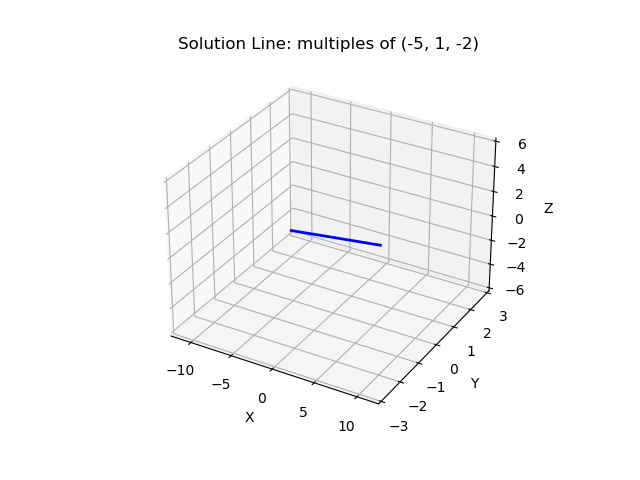
\includegraphics[width=0.8\columnwidth]{figs/solvek.png}
   \caption{}
   \label{}
   \end{figure}
\end{frame}






\begin{frame}[fragile]
    \frametitle{Code - C}
    \begin{lstlisting}
#include <stdio.h>

#define ROWS 3
#define COLS 4

// Simple row reduction for 3x4 augmented matrix
void row_reduce(double A[ROWS][COLS]) {
    // Eliminate below pivot (0,0)
    if (A[0][0] != 0) {
        for (int i = 1; i < ROWS; i++) {
            double factor = A[i][0] / A[0][0];
            for (int j = 0; j < COLS; j++) {
                A[i][j] -= factor * A[0][j];
            }
        }
    }



    \end{lstlisting}
    \end{frame}

    \begin{frame}[fragile]
    \frametitle{Code - C}
    \begin{lstlisting}
    // Eliminate below pivot (1,1)
    if (A[1][1] != 0) {
        for (int i = 2; i < ROWS; i++) {
            double factor = A[i][1] / A[1][1];
            for (int j = 0; j < COLS; j++) {
                A[i][j] -= factor * A[1][j];
            }
        }
    }
}


\end{lstlisting}
\end{frame}

\begin{frame}[fragile]
    \frametitle{Code - Python(with shared C code)}
    The code to obtain the required plot is
    \begin{lstlisting}
import ctypes
import numpy as np
import matplotlib.pyplot as plt

# --- Load shared library ---
lib = ctypes.CDLL("./solver.so")

# Define ctypes type
Mat3x4 = (ctypes.c_double * 4) * 3
lib.row_reduce.argtypes = [Mat3x4]
lib.row_reduce.restype = None

# --- Step 1: Build augmented matrix with variable k ---
k = 11  # try different k values here
A4 = Mat3x4()
\end{lstlisting}
\end{frame}
\begin{frame}[fragile]
\frametitle{Code - Python(with shared C code)}
\begin{lstlisting}
A4[0][:] = (1, k, 3, 0)
A4[1][:] = (3, k, -2, 0)
A4[2][:] = (2, 4, -3, 0)

print("Original augmented matrix:")
for row in A4:
    print([float(x) for x in row])

# --- Step 2: Row-reduce using C ---
lib.row_reduce(A4)

print("\nRow-reduced augmented matrix:")
reduced = np.array([[A4[i][j] for j in range(4)] for i in range(3)], dtype=float)
print(reduced)



\end{lstlisting}
\end{frame}

\begin{frame}[fragile]
\frametitle{Code - Python(with shared C code)}
\begin{lstlisting}
# --- Step 3: Check rank (ignoring last column) ---
coeff_matrix = reduced[:, :3]
rank = np.linalg.matrix_rank(coeff_matrix)
print("\nRank of coefficient matrix =", rank)

if rank == 3:
    print("Only trivial solution.")
    exit()

# --- Step 4: Solve system (from reduced form) ---
# From reduced system when k=11:
# Row2: 2y + z = 0 -> z = -2y
# Row1: x + 11y + 3z = 0 -> x = -5y
solution_vec = np.array([-5.0, 1.0, -2.0])
print("Solution vector:", solution_vec)


\end{lstlisting}
\end{frame}

\begin{frame}[fragile]
\frametitle{Code - Python(with shared C code)}
\begin{lstlisting}
# Ratio
x, y, z = solution_vec
ratio = (x * z) / (y * y)
print("xz / y^2 =", ratio)

# --- Step 5: Plot solution line ---
t_vals = np.linspace(-2, 2, 200)
points = t_vals[:, None] * solution_vec[None, :]

fig = plt.figure()
ax = fig.add_subplot(111, projection="3d")
ax.plot(points[:, 0], points[:, 1], points[:, 2], "b-", linewidth=2)
ax.set_xlabel("X"); ax.set_ylabel("Y"); ax.set_zlabel("Z")
ax.set_xlim([-12, 12]); ax.set_ylim([-3, 3]); ax.set_zlim([-6, 6])
ax.set_title("Solution Line: multiples of (-5, 1, -2)")
plt.savefig("solvek.png")
plt.show()



\end{lstlisting}
\end{frame}




\begin{frame}[fragile]
\frametitle{Code - Python only}
\begin{lstlisting}
import numpy as np
import matplotlib.pyplot as plt

# ---- Set k(solving with k as variable requires some concepts like nullspace which aren't taught yet) ----
k = 11.0   # change this to any real value

# ---- Build augmented matrix ----
A = np.array([
    [1, k,  3, 0],
    [3, k, -2, 0],
    [2, 4, -3, 0]
], dtype=float)

print("Original augmented matrix:")
print(A, "\n")

\end{lstlisting}
\end{frame}

\begin{frame}[fragile]
\frametitle{Code - Python only}
\begin{lstlisting}
# ---- Row reduction ----
# Step 1: eliminate below pivot (0,0)
if A[0,0] != 0:
    A[1] = A[1] - (A[1,0]/A[0,0])*A[0]
    A[2] = A[2] - (A[2,0]/A[0,0])*A[0]

# Step 2: eliminate below pivot (1,1)
if A[1,1] != 0:
    A[2] = A[2] - (A[2,1]/A[1,1])*A[1]

print("Row reduced matrix:")
print(A, "\n")

# ---- Check rank ----
rank = np.linalg.matrix_rank(A[:,:3])
print("rank =", rank)


\end{lstlisting}
\end{frame}

\begin{frame}[fragile]
\frametitle{Code - Python only}
\begin{lstlisting}
if rank == 3:
    print("Only trivial solution.")
else:
    # For k=11, reduced system gives:
    # 2y + z = 0 -> z = -2y
    # x + 11y + 3z = 0 -> x = -5y
    y = 1
    x = -5*y
    z = -2*y
    solution_vec = np.array([x,y,z], dtype=float)
    print("Solution vector:", solution_vec)

    ratio = (x*z)/(y*y)
    print("xz / y^2 =", ratio)


\end{lstlisting}
\end{frame}

\begin{frame}[fragile]
\frametitle{Code - Python only}
\begin{lstlisting}
    # ---- Plot the solution line ----
    t = np.linspace(-2, 2, 200)
    line = np.outer(t, solution_vec)

    fig = plt.figure()
    ax = fig.add_subplot(111, projection="3d")
    ax.plot(line[:,0], line[:,1], line[:,2], 'b-')
    ax.set_xlabel("X"); ax.set_ylabel("Y"); ax.set_zlabel("Z")
    ax.set_title(f"Solution line for k={k}")
    plt.savefig("newsolvek.png")
    plt.show()


\end{lstlisting}
\end{frame}
\end{document}
